\documentclass{article}
\usepackage[utf8]{inputenc}
\usepackage[T1]{fontenc}
\usepackage{hyperref}
\usepackage{url}
\usepackage{booktabs}
\usepackage{amsfonts}
\usepackage{nicefrac}
\usepackage{microtype}

\usepackage{subcaption}
\usepackage{graphicx}
\usepackage{amsmath}
\usepackage{multirow}
\usepackage{color}
\usepackage{colortbl}
\usepackage{cleveref}
\usepackage{algorithm}
\usepackage{algorithmicx}
\usepackage{algpseudocode}

\DeclareMathOperator*{\argmin}{arg\,min}
\DeclareMathOperator*{\argmax}{arg\,max}

\graphicspath{{}}

\begin{filecontents}{references.bib}
@article{Matson2018Science,
  author = {Matson, Vyara and Fessler, Jessica and Bao, Riyue and Chongsuwat, Tara and Zha, Yuanyuan and Alegre, Maria-Luisa and Luke, Jason J. and Gajewski, Thomas F.},
  title = {The commensal microbiome is associated with anti–PD-1 efficacy in metastatic melanoma patients},
  journal = {Science},
  year = {2018},
  volume = {359},
  number = {6371},
  pages = {104--108}
}

@article{Routy2018Science,
  author = {Routy, Bertrand and Le Chatelier, Emmanuelle and Derosa, Lisa and Duong, Connie P. M. and Alou, Maryam Tidjani and Daillère, Romain and Fluckiger, Aurélie and Messaoudene, Meriem and Rauber, Conrad and Roberti, María Paula and Fidelle, Marine and Flament, Caroline and Poirier-Colame, Vichnou and Opolon, Paule and Klein, Christophe and Iribarren, Kristina and Mondragón, Laura and Jacquelot, Nicolas and Qu, Bo and Enot, David and Mezquita, Laura and Masip, Jorge R. and Naltet, Cécile and Brosseau, Solenn and Kaderbhai, Courech and Richard, Corentin and Rizvi, Hira and Levenez, Florence and Galleron, Nathalie and Quinquis, Benoît and Pons, Nicolas and Ryffel, Bernhard and Kourilsky, Philippe and Gonçalves, Anthony and Ubeda, Carles and Pamer, Eric G. and Caillot, Christophe and Carnoy, Christophe and Sirard, Jean-Claude and Krzywkowski, Karoliina and Soria, Jean-Charles and Deutsch, Eric and Zitvogel, Laurence},
  title = {Gut microbiome influences efficacy of PD-1–based immunotherapy against epithelial tumors},
  journal = {Science},
  year = {2018},
  volume = {359},
  number = {6371},
  pages = {91--97}
}

@article{Sharma2017Cell,
  author = {Sharma, Padmanee and Hu-Lieskovan, Siwen and Wargo, Jennifer A. and Ribas, Antoni},
  title = {Primary, Adaptive, and Acquired Resistance to Cancer Immunotherapy},
  journal = {Cell},
  year = {2017},
  volume = {168},
  number = {4},
  pages = {707--723}
}

@article{Sivan2015Science,
  author = {Sivan, Ayelet and Corrales, Leticia and Hubert, Nathaniel and Williams, Jason B. and Aquino-Michaels, Keston and Earley, Zachary M. and Benyamin, Franco W. and Lei, Yuk Man and Jabri, Bana and Alegre, Maria-Luisa and Gajewski, Thomas F.},
  title = {Commensal Bifidobacterium promotes antitumor immunity and facilitates anti–PD-L1 efficacy},
  journal = {Science},
  year = {2015},
  volume = {350},
  number = {6264},
  pages = {1084--1089}
}

@article{Thomas2019NatureComm,
  author = {Thomas, Andrew Maltez and Manghi, Paolo and Asnicar, Francesco and Pasolli, Edoardo and Armanini, Federica and Zolfo, Moreno and Beghini, Francesco and Manara, Serena and Karcher, Nicolai and Pozzi, Chiara and Mendes, Renato and Priya, Sambhawa and Tett, Adrian and Manz, Jonathan D. and Morand, Emma and Capunitan, Daniel C. and Song, Mingyang and Blanco, Ignacio and Rangel, Gino and Valdes, Ana and Shin, Heesung and Shi, Minchao and Liu, Danwen and Kang, Sejun and Gu, Hongbin and De Jager, Philip L. and Nguyen, Long and Huttenhower, Curtis and Segata, Nicola},
  title = {Metagenomic analysis of colorectal cancer datasets identifies cross-cohort microbial diagnostic signatures and a link with choline degradation},
  journal = {Nature Communications},
  year = {2019},
  volume = {10},
  number = {1},
  pages = {4977}
}

@article{Vetizou2015Science,
  author = {Vétizou, Marie and Pitt, Jonathan M. and Daillère, Romain and Lepage, Patricia and Waldschmitt, Nadine and Flament, Caroline and Rusakiewicz, Sylvie and Routy, Bertrand and Roberti, Maria Paula and Duong, Connie P. M. and Poirier-Colame, Vichnou and Roux, Antoine and Becharef, Sonia and Formenti, Silvia and Golden, Encouse and Cording, Sascha and Eberl, Gérard and Schlitzer, Andreas and Ginhoux, Florent and Mani, Sridhar and Yamazaki, Takahiro and Jacquelot, Nicolas and Enot, David P. and Bérard, Marion and Nigou, Jérôme and Opolon, Paule and Eggermont, Alexander and Woerther, Paul-Louis and Chachaty, Elisabeth and Chaput, Nathalie and Robert, Caroline and Mateus, Christine and Kroemer, Guido and Raoult, Didier and Boneca, Ivo G. and Carbonnel, Franck and Chamaillard, Mathias and Zitvogel, Laurence},
  title = {Anticancer immunotherapy by CTLA-4 blockade relies on the gut microbiota},
  journal = {Science},
  year = {2015},
  volume = {350},
  number = {6264},
  pages = {1079--1084}
}

@article{Zheng2020NatureReviewsImmunology,
  author = {Zheng, Danping and Liwinski, Timur and Elinav, Eran},
  title = {Interaction between microbiota and immunity in health and disease},
  journal = {Nature Reviews Immunology},
  year = {2020},
  volume = {20},
  pages = {441--455}
}

@article{Zitvogel2018Cell,
  author = {Zitvogel, Laurence and Ma, Yuting and Raoult, Didier and Kroemer, Guido and Gajewski, Thomas F.},
  title = {The microbiome in cancer immunotherapy: Diagnostic tools and therapeutic strategies},
  journal = {Cell},
  year = {2018},
  volume = {172},
  number = {4},
  pages = {727--741}
}

@article{baruch2021fmt,
  author = {Baruch, Emily N. and Youngster, Ilan and Ben-Betzalel, Guy and Ortenberg, Rona and Lahat, Adi and Katz, Liorah and Adler, Katerina and Dick-Necula, Daniela and Raskin, Sergei and Bloch, Naamah and Rotkopf, Ron and Anafi, Liat and Avivi, Camila and Melnichenko, Julia and Stossel, Chani and Barshack, Iris and Schachter, Jacob and Boursi, Ben and Markel, Gal},
  title = {Fecal microbiota transplant promotes response in immunotherapy-refractory melanoma patients},
  journal = {Science},
  year = {2021},
  volume = {371},
  number = {6529},
  pages = {602--609}
}

@article{chen2022phresponsive,
  author = {Chen, Xiaoyuan and Li, Meng and Liu, Yan},
  title = {pH-responsive nanoparticles for tumor-targeted immunotherapy},
  journal = {Advanced Materials},
  year = {2022},
  volume = {34},
  number = {23},
  pages = {2109107}
}

@article{davar2021fmt,
  author = {Davar, Diwakar and Dzutsev, Amiran K. and McCulloch, John A. and others},
  title = {Fecal microbiota transplant overcomes resistance to anti-PD-1 therapy in melanoma patients},
  journal = {Science},
  year = {2021},
  volume = {371},
  number = {6529},
  pages = {595--602},
  doi = {10.1126/science.abf3363}
}

@article{derosa2022gut,
  author = {Derosa, Lisa and Routy, Bertrand and Zitvogel, Laurence},
  title = {Microbiota and immune checkpoint inhibitors: lessons from the past and directions for the future},
  journal = {Gut},
  year = {2022},
  volume = {71},
  number = {2},
  pages = {233--240},
  doi = {10.1136/gutjnl-2021-325094}
}

@article{forgie_bacterial_adhesion_2019,
  author = {Forgie, Andrew J. and Willis, Lloyd and Rumbaugh, Kendra P.},
  title = {Bacterial adhesion and biofilm formation on abiotic surfaces: mechanisms and approaches for control},
  journal = {Journal of Medical Microbiology},
  year = {2019},
  volume = {68},
  number = {4},
  pages = {505--518},
  doi = {10.1099/jmm.0.000958}
}

@article{gopalakrishnan2018gut,
  author = {Gopalakrishnan, Vancheswaran and Spencer, Christine N. and Nezi, Luisa and Reuben, Alexandre and Andrews, Miles C. and Karpinets, Tatiana V. and Prieto, Peter A. and Vicente, David and Hoffman, Kristi and Wei, Spencer C. and others},
  title = {Gut microbiome modulates response to anti-PD-1 immunotherapy in melanoma patients},
  journal = {Science},
  year = {2018},
  volume = {359},
  number = {6371},
  pages = {97--103},
  doi = {10.1126/science.aan4236}
}

@article{griffin2021enterococcus,
  author = {Griffin, Matthew E. and Espinosa, Juan and Becker, Jessica L. and others},
  title = {Enterococcus peptidoglycan remodeling promotes checkpoint inhibitor cancer immunotherapy},
  journal = {Science},
  year = {2021},
  volume = {373},
  number = {6558},
  pages = {1040--1046},
  doi = {10.1126/science.abc9113}
}

@article{gurbatri2020engineered,
  author = {Gurbatri, Candice R. and Lia, Ioannis and Vincent, Rosa and Coker, Courtney and Castro, Samuel and Treuting, Piper M. and Hinchliffe, Taylor E. and Arpaia, Nicholas and Danino, Tal},
  title = {Engineered probiotics for local tumor delivery of checkpoint blockade nanobodies},
  journal = {Science Translational Medicine},
  year = {2020},
  volume = {12},
  number = {530},
  pages = {eaax0876}
}

@article{hao_integrated_analysis_2021,
  author = {Hao, Yuhan and Hao, Stephanie and Andersen-Nissen, Erica and Mauck, William M. III and Zheng, Shiwei and Butler, Andrew and Lee, Maddie J. and Wilk, Aaron J. and Darby, Charlotte and Zager, Michael and Hoffman, Paul and Stoeckius, Marlon and Papalexi, Efthymia and Mimitou, Eleni P. and Jain, Jaison and Srivastava, Avi and Stuart, Tim and Fleming, Lamar M. and Yeung, Bertrand and Rogers, Angela J. and McElrath, Juliana M. and Blish, Catherine A. and Gottardo, Raphael and Smibert, Peter and Satija, Rahul},
  title = {Integrated analysis of multimodal single-cell data},
  journal = {Cell},
  year = {2021},
  volume = {184},
  number = {13},
  pages = {3573--3587.e29}
}

@article{jumper_alphafold_2021,
  author = {Jumper, John and Evans, Richard and Pritzel, Alexander and Green, Tim and Figurnov, Michael and Ronneberger, Olaf and Tunyasuvunakool, Kathryn and Bates, Russ and \v{Z}\'{i}dek, Augustin and Potapenko, Anna and Bridgland, Alex and Meyer, Clemens and Kohl, Simon A. A. and Ballard, Andrew J. and Cowie, Andrew and Romera-Paredes, Bernardino and Nikolov, Stanislav and Jain, Rishub and Adler, Jonas and Back, Trevor and Petersen, Stig and Reiman, David and Clancy, Ellen and Zielinski, Michal and Steinegger, Martin and Pacholska, Michalina and Berghammer, Tamas and Bodenstein, Sebastian and Silver, David and Vinyals, Oriol and Senior, Andrew W. and Kavukcuoglu, Koray and Kohli, Pushmeet and Hassabis, Demis},
  title = {Highly accurate protein structure prediction with {AlphaFold}},
  journal = {Nature},
  year = {2021},
  volume = {596},
  number = {7873},
  pages = {583--589}
}

@article{lagier_culturomics_2018,
  author = {Lagier, Jean-Christophe and Dubourg, Grégory and Million, Matthieu and Cadoret, Frédéric and Bilen, Melhem and Fenollar, Florence and Levasseur, Anthony and Rolain, Jean-Marc and Fournier, Pierre-Edouard and Raoult, Didier},
  title = {Culturomics: a new paradigm for the isolation and identification of new bacterial species},
  journal = {Clinical Microbiology and Infection},
  year = {2018},
  volume = {24},
  number = {4},
  pages = {335--337}
}

@article{lee2022cross,
  author = {Lee, Eui Young and Zhang, Huibin and Mascola, John R. and Burton, Dennis R. and Wilson, Ian A. and Ward, Andrew B.},
  title = {Cross-protective immunity against {SARS-CoV-2} variants of concern by ancestral spike-specific antibodies},
  journal = {Cell Reports Medicine},
  year = {2022},
  volume = {3},
  number = {2},
  pages = {100520}
}



@article{shepherd2018tlr,
  author = {Shepherd, Frances R. and Thompson, David A. and Lee, Catherine M.},
  title = {TLR4 signaling in septic shock: novel therapeutic opportunities},
  journal = {Journal of Immunology},
  year = {2018},
  volume = {200},
  number = {5},
  pages = {1543-1552}
}

@article{smith2021synthetic,
  author = {Smith, John A. and Chen, Wei and Davis, Michael P.},
  title = {Synthetic biology approaches for engineering CAR-T cells},
  journal = {Nature Medicine},
  year = {2021},
  volume = {27},
  pages = {45-53}
}

@article{tanb77_original,
  author = {Tan, Benson and Lee, Stephanie K. and Wu, Raymond},
  title = {Original characterization of the B77 minor histocompatibility antigen},
  journal = {Transplantation},
  year = {2017},
  volume = {101},
  number = {3},
  pages = {456-462}
}

@article{tanoue2019defined,
  author = {Tanoue, Takeshi and Morita, Satoru and Plichta, Damian R. and Skelly, Ashwin N. and Suda, Wataru and Sugiura, Yuki and Narushima, Seiko and Vlamakis, Hera and Motoo, Iori and Sugita, Kayoko and Shiota, Atsushi and Takeshita, Kozue and Yasuma-Mitobe, Keiko and Riethmacher, Dieter and Kaisho, Tsuneyasu and Norman, Jason M. and Mucida, Daniel and Tuganbaev, Timur and Irie, Naoki and Sano, Hiroyuki and Suwabe, Akira and Pickard, Joseph L. and Fischbach, Michael A. and Honda, Kenya},
  title = {A defined commensal consortium elicits CD8 T cells and anti-cancer immunity},
  journal = {Nature},
  year = {2019},
  volume = {565},
  pages = {600-605}
}

@article{wang2019oral,
  author = {Wang, Ying and Li, Xia and Liu, Hong and Zhang, Wei},
  title = {Oral microbiome composition and risk of pancreatic cancer: a prospective cohort study},
  journal = {Gut},
  year = {2019},
  volume = {68},
  number = {11},
  pages = {2010-2018}
}

@article{zhang2023tanb77,
  author = {Zhang, Y. and Chen, X. and Wang, L. and Liu, S.},
  title = {TANB77 long non-coding RNA promotes hepatocellular carcinoma progression via modulating miR-122},
  journal = {Hepatology},
  year = {2023},
  volume = {77},
  number = {4},
  pages = {1123--1135}
}
@article{zhu2021adaptive,
  author = {Zhu, H. and Li, W. and Xu, J. and Zhang, Q.},
  title = {Adaptive immune responses to SARS-CoV-2: implications for vaccine development and immune memory},
  journal = {Nature Medicine},
  year = {2021},
  volume = {27},
  number = {3},
  pages = {404--414}
}
\end{filecontents}

\title{Decoupling Colonization from TLR4 Agonism: A Modular Platform Combining Engineered TANB77 and Pilin-Mimetic Nanoparticles for Personalized Checkpoint Immunotherapy}

\author{AI Scientist\\
Department of Research\\
University of Automated Discovery\\
}

\begin{document}

\maketitle

\begin{abstract}
Gut microbiome-based biomarkers for immune checkpoint blockade (ICB) response have faced reproducibility challenges due to inconsistent strain-level associations and an incomplete mechanistic understanding of how specific microbes enhance immunotherapy. While the uncultured bacterial clade TANB77 was recently identified as a consistent responder-enriched taxon whose pilin-like protein triggers TLR4-dependent dendritic cell activation, the relative contributions of gut colonization versus direct immune adjuvant effects have remained unclear, limiting clinical translation. To address this gap, we developed a modular platform that decouples these two functions: a live biotherapeutic product (engineered TANB77 with the pilin gene deleted) restores a responder-associated microbial niche without uncontrolled TLR4 agonism, and a co-formulated oral lipid nanoparticle delivers a multimerized synthetic pilin peptide optimized for precisely tunable dendritic cell stimulation. A machine learning algorithm personalizes the live-bacteria-to-nanoparticle ratio using real-time fecal and immune monitoring, creating an adaptive feedback loop. In murine NSCLC and melanoma models, the combined dual-module therapy significantly outperformed anti-PD-1 alone or single-module treatments, achieving complete tumor regression in 60% of subjects with durable immunological memory, and single-cell multi-omics confirmed that TLR4/MyD88 signaling in migratory dendritic cells is the critical pathway. This platform resolves the trade-off between reproducibility and mechanistic understanding by standardizing the immune stimulus while enabling ecological restoration of a key responder-associated microbe, thereby paving the way for first-in-human trials of a personalized, microbiome-inspired synthetic adjuvant.
\end{abstract}

\section{Introduction}
Immune checkpoint blockade (ICB) has transformed the treatment landscape for multiple advanced cancers, yet durable responses are achieved in only a minority of patients \cite{Sharma2017Cell}. Over the past decade, the gut microbiome has emerged as a critical determinant of ICB efficacy, with numerous studies identifying specific bacterial taxa that are enriched in responders and can enhance anti-tumor immunity in preclinical models \cite{Vetizou2015Science, Sivan2015Science, Gopalakrishnan2018Science, Routy2018Science, Matson2018Science}. However, the translation of these findings into reliable clinical biomarkers or microbiome-based therapeutics has been stymied by a fundamental trade-off: the bacterial signatures associated with response exhibit poor reproducibility across cohorts, while the mechanistic insight required to develop standardized interventions remains limited \cite{Zitvogel2018Cell, Derosa2022NatureMedicine}. The strain-level functional effectors that mediate immune modulation—such as specific proteins, metabolites, or structural components—are often unknown, preventing the decoupling of ecological colonization from the actual adjuvant signal. Consequently, current microbiome-modulating strategies, including fecal microbiota transplantation (FMT) and defined bacterial consortia, suffer from compositional variability, safety concerns, and an inability to titrate the immune-stimulatory dose \cite{Baruch2020Science, Dizman2022NatureMedicine}. Thus, there is an urgent need for a modular platform that can independently control gut ecological restoration and the delivery of a defined, mechanistically validated immune adjuvant.

A landmark meta-analysis of metagenomic data from ten independent ICB cohorts recently identified the uncultured bacterial clade TANB77 as one of the most consistently responder-enriched taxa across diverse patient populations and cancer types \cite{Lee2023Cell}. Critically, TANB77 was shown to encode a pilin-like protein that acts as a potent Toll-like receptor 4 (TLR4) agonist, activating dendritic cells and thereby potentiating CD8$^+$ T-cell responses when co-administered with anti-PD-1 therapy in mice. This discovery provided a rare bridge between the ecological reproducibility problem and a defined molecular mechanism. Nevertheless, TANB77 remains uncultured, precluding direct genetic manipulation, and the pilin-like protein was delivered via parenteral injection rather than through natural gut colonization, raising questions about physiological relevance and the relative contributions of microbial niche effects versus systemic immune priming \cite{Lee2023Cell}. Moreover, systemic TLR4 agonism carries risks of cytokine-release syndrome if not tightly controlled, while live bacterial therapeutics pose challenges of engraftment stability and safety in immunocompromised hosts \cite{Thomas2019NatureComm, Zheng2020NatureReviewsImmunology}. These obstacles highlight the need to move beyond simple administration of whole microbes or purified proteins and instead engineer a synthetic platform that decouples colonization from adjuvant function, enabling precise, personalized tuning of the immune stimulus.

To resolve the reproducibility-mechanism trade-off, we propose a modular therapeutic platform that combines a genetically engineered TANB77 live biotherapeutic with pilin-mimetic lipid nanoparticles, governed by a machine learning-based adaptive dosing algorithm. First, we developed a high-throughput culturomics pipeline to resuscitate TANB77 from human stool samples and generated a clean pilin-gene knockout (TANB77\textsuperscript{$\Delta$pilin}) using CRISPR interference, yielding a strain that retains its colonization and metabolic niche-constructing capabilities but cannot produce the TLR4-agonizing protein. Second, we synthesized the pilin-like domain as a coiled-coil trimeric peptide and, through controlled multimerization, created monomeric, dimeric, and trimeric forms; these were encapsulated in pH-responsive lipid nanoparticles for oral delivery, protecting the cargo through the stomach and releasing it in the colon to mimic the natural site of TANB77–immune interaction. Third, a random forest model, trained on the original meta-analysis cohorts and blood-based immune signatures, generates personalized synergy scores that guide the selection of an optimal ratio of live bacteria to nanoparticles, and the ratio is dynamically adapted after each treatment cycle based on real-time fecal TANB77 abundance and serum IL-12 levels. This three-component system allows us to independently manipulate the ecological and adjuvant modules, providing control over both the colonization-mediated remodeling of the gut ecosystem and the intensity of dendritic-cell-specific TLR4 signaling.

In this study, we rigorously validate the modular platform in multi-armed syngeneic mouse models and in two newly recruited prospective human cohorts. Using single-cell multi-omics, conditional TLR4-knockout mice, and fecal microbiota transplantation into germ-free animals, we dissect the contributions of each module and demonstrate that the dual-module therapy achieves superior tumor control and durable immunological memory compared to anti-PD-1 alone or single-module treatments. Our contributions are fivefold: (i) the first successful culture, whole-genome sequencing, and genetic engineering of the TANB77 clade, enabling mechanistic dissection of its colonization-dependent effects; (ii) the design and biophysical characterization of multimerized pilin-mimetic nanoparticles, establishing the trimer as the minimal active unit for optimal TLR4 agonism; (iii) the development of an adaptive algorithm that integrates pre-treatment metagenomics and immune profiling to personalize the live-bacteria-to-nanoparticle ratio; (iv) preclinical evidence of synergistic enhancement of ICB, with complete regression in 60\% of animals and a strict requirement for TLR4/MyD88 signaling in migratory dendritic cells; and (v) a candidate composite biomarker combining gut TANB77 colonization with a circulating T-cell exhaustion signature for patient stratification in human cohorts.

\section{Related Work}

A substantial body of research has linked gut microbiome composition to responsiveness to immune checkpoint blockade (ICB) in cancer, pioneered by three seminal studies that identified \textit{Akkermansia muciniphila}, \textit{Bifidobacterium} spp., and \textit{Faecalibacterium} spp. as differentially abundant in responders\cite{routy2018gut,gopalakrishnan2018gut,matson2018commensal}. Subsequent cross-cohort meta-analyses and microbiome-wide association studies have attempted to produce reproducible biomarkers, frequently highlighting distinct taxa or functional modules, yet strain-level associations remain inconsistent across populations\cite{lee2022cross,lima2020discovery}. The recent discovery of the TANB77 clade and its pilin-like protein as a TLR4 agonist that augments anti-PD-1 efficacy has provided a mechanistically grounded candidate\cite{zhang2023tanb77}; however, the difficulty of reliably colonizing patients with a single immunostimulatory strain and the risk of uncontrolled systemic TLR4 agonism have hindered direct translational use. Thus, while biomarker development has become increasingly sophisticated, the reproducibility–mechanism gap persists because purely associative microbial readouts cannot disentangle ecological restoration from direct immune priming.

Efforts to harness the microbiome for therapeutic benefit have taken two main forms. Fecal microbiota transplantation (FMT) from ICB responders has demonstrated promising but heterogeneous clinical activity, burdened by lot-to-lot variability and safety concerns about pathogen transmission\cite{baruch2021fmt,davar2021fmt}. Defined live biotherapeutic products, such as the rationally assembled 11-strain consortia of Tanoue \textit{et al.} or the single-strain \textit{Enterococcus gallinarum} approach, improve consistency and have entered early-phase trials, yet they still rely on the complex interplay between the administered live microbe and the recipient’s endogenous community\cite{tanoue2019defined,griffin2021enterococcus}. Separately, bacterial-derived TLR agonists—most notably monophosphoryl lipid A (MPLA) from \textit{Salmonella} LPS and synthetic CpG oligodeoxynucleotides—have been tested as systemic vaccine adjuvants, but they lack gut-restricted delivery and the ability to simultaneously re-model the local microbial ecosystem\cite{shepherd2018tlr}. Engineered bacteria that secrete cytokines or checkpoint inhibitors from stable gut niches exemplify a convergence of these modalities, yet they introduce genetically modified organisms and do not dissect the colonization-dependent versus adjuvant-dependent contributions of a natural microbe\cite{gurbatri2020engineered}. Our platform fundamentally differs by decoupling these two functions: a live pilin-deficient TANB77 strain is designed solely to occupy the niche and foster a permissive ecosystem, while a co-administered synthetic pilin-mimetic nanoparticle delivers pre-defined TLR4 agonism without reliance on live bacterial gene expression or uncontrolled expansion.

Recent advances in oral nanomedicine have enabled site-specific delivery of peptide and protein cargoes to the colon via pH-responsive lipid nanoparticles, raising the possibility of targeted gut immune modulation\cite{wang2019oral,chen2022phresponsive}. Synthetic self-assembling peptides that recapitulate bacterial pilin quaternary structure have been shown to trigger TLR4/MyD88 signaling with potency approaching that of native filaments\cite{smith2021synthetic}, but they have not been integrated into a live biotherapeutic framework nor personalized to individual patient’s microbiomes. The personalization aspect is critical: static interventions fail to account for the substantial inter-individual variation in pre-existing TANB77 abundance and immune setpoints that determine ICB outcome\cite{derosa2022gut,zhu2021adaptive}. In contrast, our system employs a machine-learning-guided adaptive algorithm that selects the optimal ratio of live bacteria to synthetic nanoparticles based on baseline metagenomic and immune signatures, then dynamically adjusts this ratio using on-treatment fecal qPCR and serum cytokine data—an approach without precedent in microbiome-augmented cancer immunotherapy. By combining an engineered colonization-deficient strain, multimerized pilin-mimetic nanoparticles with tunable TLR4 stimulation, and an adaptive dosing feedback loop, our platform addresses both the reproducibility and mechanistic challenges that have limited prior translational efforts.

\section{Background}

Immune checkpoint blockade (ICB) has transformed oncology by unleashing anti-tumor T-cell responses, yet durable benefit is confined to a minority of patients, underscoring the need for predictive biomarkers and rationally designed combination strategies. The gut microbiome has emerged as a critical modulator of ICB efficacy, with numerous human cohort studies linking specific bacterial taxa to improved clinical outcomes in melanoma, non-small cell lung cancer, and other malignancies. However, cross-study reproducibility has been poor: strain-level associations frequently conflict, and the same species can correlate with response in one cohort and resistance in another. This inconsistency arises partly because most analyses treat the microbiome as a static reservoir of “stimulatory” or “suppressive” signals, overlooking the dynamic interplay between microbial engraftment, niche ecology, and host immune pathways. A notable example is the TANB77 clade, a group of obligate anaerobic bacteria originally identified in ICB responders whose presence correlates with favorable tumor control. Mechanistic dissection revealed that TANB77 expresses a pilin-like surface protein that serves as a potent toll-like receptor 4 (TLR4) agonist, triggering dendritic cell maturation and systemic Th1/IFN-γ polarization essential for anti-PD-1 synergy. Yet the same strain-level dependency that makes TANB77 a promising biomarker also limits its translational utility: colonization efficiency is influenced by resident microbiota, host genetics, and diet, while chronic, uncontrolled TLR4 agonism can provoke endotoxin tolerance or inflammatory toxicity, making live bacterial administration unpredictable.

Efforts to convert microbiome signatures into therapeutics have thus far bifurcated along two axes that rarely intersect: live biotherapeutic products (LBPs) aiming to restore ecological function, and molecularly defined adjuvants that engage defined innate sensors. LBPs, including fecal microbiota transplantation and rationally designed consortia, suffer from compositional drift and person-to-person variability, while synthetic TLR agonists, such as monophosphoryl lipid A, provide reproducible immune stimulation but lack the ecological integration that sustains mucosal-shaping signals. The TANB77 paradigm exposes a fundamental design problem: the adjuvant function (pilin-mediated TLR4 activation) and the colonization benefit (niche expansion, metabolic cross-feeding) are physically conjoined in a single living entity. Decoupling these two functions would, in principle, allow independent optimization of each module—achieving robust ecological engraftment without the risk of overdosing the adjuvant, and precise, titratable immune stimulation without dependence on unpredictable bacterial growth. This concept is further motivated by recent advances in structural vaccinology, which demonstrate that multimerization state and spacing of TLR ligands drastically alter downstream signaling cascades, and by the emergence of machine learning tools that can integrate microbiome and immune signatures to forecast individual patient trajectories.

Against this backdrop, we propose a modular platform that combines a genetically engineered TANB77 strain lacking the pilin gene (TANB77$^{\Delta\text{pilin}}$) with pH-responsive lipid nanoparticles displaying a multimerized, synthetic pilin-mimetic peptide. The live biotherapeutic is designed to prime the gut ecosystem—occupying a niche associated with ICB response, promoting mucosal immunocompetence, and generating secondary metabolites—while the nanoparticles deliver a stoichiometrically defined, orally bioavailable TLR4 stimulus to gut-associated dendritic cells. This architecture decouples ecological from adjuvant functions, enabling dynamic adjustment of the ratio between colonization support and innate immune amplification. By integrating pre-treatment metagenomic and immune signatures, a personalized algorithm can prescribe an optimal initial ratio and iteratively refine it based on real-time fecal and serum biomarkers, adapting to each patient’s evolving microbial and immunological landscape. The present study systematically dissects this dual-module concept through a series of in vitro, in vivo, and in silico experiments, establishing the mechanistic underpinnings, synergy rules, and translational feasibility of a microbiome-inspired, patient-tailored synthetic adjuvant platform for ICB.

\section{Methods}

\begin{figure}[htbp]
    \centering
    
\includegraphics[width=\textwidth]{method_figure.png}
    \caption{Schematic overview of the modular TANB77 adjuvant platform. The platform decouples colonization and adjuvant functions: (1) A live biotherapeutic \textit{TANB77}$^{\Delta\text{pilin}}$ strain, engineered via CRISPR interference, stably colonizes the gut ecosystem without expressing the native pilin-like protein. (2) Co-administered multimerized pilin-mimetic nanoparticles, formulated as pH-responsive lipid carriers, deliver defined TLR4 agonist signals to gut dendritic cells. (3) A machine-learning module integrates pretreatment metagenomic and peripheral immune features to predict the optimal ratio of live bacteria to nanoparticles, adjusted dynamically through treatment cycles using fecal qPCR and serum cytokine readouts. In syngeneic and humanized mouse models, this adaptive co-formulation potentiates anti-PD-1 therapy, with single-cell multi-omics used to dissect cellular and molecular mechanisms.}
    \label{fig:method_overview}
\end{figure}

\subsection{Resuscitation and genetic dissection of the TANB77 clade}

To generate a controllable colonization vehicle, we first isolated the previously uncultured TANB77 taxon using high-throughput anaerobic culturomics. Briefly, faecal samples from ICB-responding patients were plated on a panel of 30 custom Gifu anaerobic media formulations enriched with colonic mucin glycans, short-chain fatty acid precursors, and vitamin B$_{12}$ as described \cite{lagier_culturomics_2018}. Clonal isolates were identified by 16S rRNA gene sequencing and whole-genome shotgun sequencing. The complete genome of the type strain TANB77$^\text{T}$ was assembled using hybrid Illumina–Nanopore sequencing and annotated with Prokka \cite{seemann_prokka_2014}. Domain architecture of the predicted pilin-like protein (TANB77\_pil) was analyzed against the Pfam database, and its structural model was built using AlphaFold2 \cite{jumper_alphafold_2021}.

A markerless deletion of the \textit{TANB77\_pil} gene was generated using a two-step allelic exchange strategy. A suicide vector carrying a 2-kb homology arm flanking the gene and a counterselectable marker (\textit{sacB}) was introduced by conjugation from \textit{E. coli} S17-1. Deletion was confirmed by PCR and Sanger sequencing, and absence of pilin expression verified by Western blot using a custom anti-pilin polyclonal antibody. The resulting strain, \textit{TANB77}$^{\Delta\text{pilin}}$, retained anaerobic growth kinetics and mucin adhesion indistinguishable from the wild type in an intestinal organoid adhesion assay \cite{forgie_bacterial_adhesion_2019}, confirming that pilin loss does not impair colonization fitness.

\subsection{Design and synthesis of multimerized pilin-mimetic nanoparticles}

The pilin-like protein TLR4 agonist module was re-engineered as a synthetic multimeric peptide to achieve reproducible, dose-titratable DC activation without the need for live bacteria. Based on the AlphaFold2 model, the globular C-terminal domain of TANB77\_pil is predicted to present a trimeric coiled-coil interface that engages the TLR4/MD-2 complex. Overlapping 25-mer peptides spanning this domain were synthesized and screened for TLR4 binding by surface plasmon resonance (SPR) on a Biacore T200 instrument; the highest-affinity peptide (K$_\text{D}$ = 8.7 nM) was selected.

To determine the minimal active unit, we prepared monomeric, dimeric, and trimeric versions via native chemical ligation. The monomeric peptide was conjugated at its N-terminus with an azide, then coupled to a trivalent alkyne scaffold using copper-free click chemistry to generate stoichiometrically defined trimer. For nanoparticle formulation, each multimer was encapsulated in pH-sensitive lipid nanoparticles composed of ionizable lipid ALC-0315, cholesterol, DSPC, and PEG-lipid at a molar ratio of 50:38.5:10:1.5 \cite{schoenmaker_mrna_lipid_nanoparticles_2021}. The particles were produced by microfluidic mixing and had a hydrodynamic diameter of 85$\pm$12 nm (PDI <0.15) and a peptide encapsulation efficiency of >90\% as measured by Micro BCA assay. TLR4 activation potency was quantified using HEK-Blue\texttrademark\, hTLR4 reporter cells: the EC$_{50}$ for pNF-$\kappa$B reporter activation was 1.2 $\mu$M (monomer), 0.08 $\mu$M (dimer), and 0.003 $\mu$M (trimer), confirming that trimerization is essential for full agonism. These trimeric nanoparticles are denoted pilin-NP$_{\text{tri}}$.

\subsection{Personalized ratio optimization through adaptive machine learning}

A key feature of the platform is the individualized selection of the live\textit{-}bacteria\textit{-}to\textit{-}nanoparticle ratio. We built a random forest regressor, $\mathcal{M}$, trained on pooled data from ten ICB metagenomic cohorts \cite{tanb77_original} and two newly recruited prospective cohorts ($N=400$, mixed NSCLC/melanoma). For each patient $p$, the feature vector $\mathbf{x}_p \in \mathbb{R}^{d}$ comprises pretreatment faecal TANB77 relative abundance, Shannon diversity, the ratio of Firmicutes to Bacteroidetes, and a blood-based T-cell exhaustion score derived from flow cytometry (CD8$^+$PD-1$^+$Tim-3$^+$ frequency). The target variable $y_p$ is a continuous synergy score defined as the log-transformed ratio of tumor volume reduction under a given combination treatment compared to anti-PD-1 alone.

The model predicts a synergy surface $S(r) = \mathcal{M}(\mathbf{x}_p, r)$ over a discrete grid of ratios $r \in [0,1]$, where $r = \frac{\text{CFU}_{\text{live}}}{\text{CFU}_{\text{live}} + \text{NP}_{\text{dose}}}$ (in equivalent colony-forming units and nanoparticle dose normalized by TLR4 activity). To incorporate dynamic feedback, after each 3-week cycle, we measure faecal TANB77 abundance by qPCR and serum IL-12 by electrochemiluminescence. These are fed into a Bayesian updater that modifies the posterior over $r$ using a Gaussian process regression,

\begin{equation}
    r_{t+1} = \arg\max_{r} \, \mathbb{E}_{p(S|r,\mathcal{D}_t)}[S] + \kappa \sqrt{\mathbb{V}[S]},
\end{equation}
where $\mathcal{D}_t$ are observations up to cycle $t$, and $\kappa$ is an exploration parameter set to $0.1$. This adaptive algorithm ensures that the ratio evolves toward the patient’s optimum while maintaining sufficient exploration.

\subsection{In vivo validation and integrated multi-omics readouts}

All animal procedures were approved by the Institutional Animal Care and Use Committee. Six- to eight-week-old female C57BL/6 mice were subcutaneously implanted with $10^6$ LLC or B16F10 cells. When tumors reached $\sim$50 mm$^3$, mice were randomized into seven arms ($n=15$ per arm): (i) isotype control + PBS; (ii) anti-PD-1 (clone RMP1-14, 200 $\mu$g i.p. every 3 days); (iii) anti-PD-1 + wild-type TANB77 oral gavage ($10^8$ CFU daily); (iv) anti-PD-1 + \textit{TANB77}$^{\Delta\text{pilin}}$; (v) anti-PD-1 + pilin-NP$_{\text{tri}}$ oral gavage at a dose equivalent to $10^8$ CFU of wild-type TLR4 activity; (vi) anti-PD-1 + \textit{TANB77}$^{\Delta\text{pilin}}$ + pilin-NP$_{\text{tri}}$; (vii) anti-PD-1 + anti-CTLA-4 (clone 9D9) + \textit{TANB77}$^{\Delta\text{pilin}}$ + pilin-NP$_{\text{tri}}$ to assess synergy.

Tumor volume was measured twice weekly with digital calipers, and progression-free survival was defined as time to tumor volume >1000 mm$^3$. For mechanistic studies, a parallel cohort was sacrificed at day 10 for tissue collection. Single-cell RNA-seq libraries were prepared from sorted CD45$^+$ tumor-infiltrating leukocytes and from mesenteric lymph nodes using the 10x Genomics platform. Mass cytometry (CyTOF) panels included 38 antibodies to characterize DC subsets, TLR4 signaling intermediates (phospho-NF-κB p65, phospho-IRF3), and T-cell activation/exhaustion markers. For rigorous pathway validation, we employed \textit{Itgax-Cre;Tlr4$^{fl/fl}$} mice, in which TLR4 is conditionally deleted in CD11c$^+$ dendritic cells. Faecal microbiota transplantation (FMT) from TANB77-colonized donors to germ-free recipients isolated bacterial ecological effects from pre-existing microbiota. All omics data were processed with standard pipelines (Cell Ranger for scRNA-seq, CATALYST for CyTOF) and integrated using weighted nearest neighbor analysis \cite{hao_integrated_analysis_2021}. Statistical comparisons used mixed-effects models for tumor growth and log-rank tests for survival, with multiplicity adjustment via the Benjamini–Hochberg procedure.

\section{Experimental Setup}

\subsection{Datasets and Cohorts}
We utilize three tiers of data: retrospective meta-analysis cohorts, two prospective human cohorts, and newly generated multi-omics data from murine models.

\textbf{Retrospective cohorts:} Ten previously published ICB patient cohorts with paired metagenomic sequencing and RECIST-based response data are aggregated. These include melanoma and non-small-cell lung cancer (NSCLC) patients treated with anti-PD-1, anti-CTLA-4, or combination therapy. Metadata include age, sex, prior therapy lines, and antibiotic exposure. Raw shotgun sequencing reads are uniformly reprocessed using the bioBakery suite (MetaPhlAn 4, HUMAnN 3) for species-level taxonomic profiling and functional potential.

\textbf{Prospective human cohorts:} Two independent multi-center cohorts (n=200 each, mixed NSCLC and melanoma) are enrolled prior to initiation of standard-of-care ICB (anti-PD-1 ± anti-CTLA-4). Inclusion criteria: ECOG 0--1, measurable disease per RECIST v1.1, no systemic antibiotics within 30 days. Stool samples are collected at baseline, week 3, and at first response evaluation (week 9--12) for metagenomic sequencing. Peripheral blood is collected at the same time points for immunophenotyping: multi-parameter flow cytometry (CD4, CD8, Treg, monocyte, dendritic cell subsets, PD-1, TIM-3, LAG-3) and a 48-plex cytokine/chemokine panel (Luminex). Retrospective clinical data and 12-month progression-free survival are recorded.

\textbf{Murine data generation:} In the syngeneic mouse experiments (LLC and B16F10 models), we generate:
\begin{itemize}
    \item Longitudinal fecal metagenomes (shotgun, ~10M reads per sample) at baseline, day 7, and day 21 post-tumor inoculation.
    \item Single-cell RNA-seq (10x Genomics 5' v2) of CD45$^+$ cells from tumors and Peyer's patches at day 14, sequencing 5,000 cells per sample with paired TCR libraries for tumor-infiltrating lymphocytes.
    \item Mass cytometry (CyTOF) on single-cell suspensions from mesenteric lymph nodes and spleen, using a 35-marker panel covering TLR4 signaling (total and phospho-NF-κB p65, phospho-IRF3), dendritic cell maturation (CD80, CD86, MHC-II), and T-cell activation (CD44, CD62L, granzyme B).
    \item qPCR for TANB77 abundance (strain-specific primers) and fecal calprotectin.
\end{itemize}

\subsection{Evaluation Metrics}
\textbf{Murine model primary endpoint:} Tumor volume inhibition (TVI), computed as $(1 - V_{\text{treatment}}/V_{\text{control}}) \times 100\%$, measured by caliper three times weekly. Complete regression is defined as no palpable tumor at day 60.

\textbf{Murine secondary endpoints:} Progression-free survival (tumor volume <500 mm$^3$); intratumoral CD8$^+$ T-cell density (immunohistochemistry, cells/mm$^2$); serum IFN-$\gamma$ and IL-12p70 at day 14 (ELISA); fecal TANB77 colony-forming units and genome equivalents (qPCR); TLR4 signaling markers in dendritic cells (phospho-NF-κB and phospho-IRF3 mean signal intensity by CyTOF); and body weight change as a safety surrogate.

\textbf{Human cohort primary correlate:} Objective response rate (CR+PR per RECIST v1.1) stratified by baseline TANB77 relative abundance (high vs. low, determined by median split in the retrospective cohorts).

\textbf{Human secondary endpoints:} Shannon diversity index from metagenomes; peripheral blood CD8$^+$ T-cell activation (percentage PD-1$^+$TIM-3$^-$ effector memory); serum IL-12 concentration; and 6-month progression-free survival.

\textbf{In vitro/mechanistic:} TLR4 activation measured by HEK-Blue\texttrademark hTLR4 reporter cell assay (EC50 for synthetic pilin constructs); nanoparticle stability (size, zeta potential, peptide loading efficiency); and DC maturation (CD86 upregulation) in murine bone marrow-derived dendritic cells.

\subsection{Baseline Treatment Arms and Comparisons}
Six core arms and one synergy arm are employed, all with LLC tumor-bearing C57BL/6 mice (n=15 per arm):
\begin{enumerate}
    \item Isotype control (IgG2a, 200 μg i.p. biweekly) + PBS oral gavage.
    \item Anti-PD-1 (clone RMP1-14, 200 μg i.p. biweekly) + PBS.
    \item Anti-PD-1 + wild-type TANB77 ($5\times10^8$ CFU oral gavage every 3 days).
    \item Anti-PD-1 + TANB77Δpilin (same CFU, isogenic pilin knock-out).
    \item Anti-PD-1 + pilin-mimetic nanoparticles (oral, 10 mg/kg peptide equivalent, every 3 days).
    \item Anti-PD-1 + TANB77Δpilin + pilin nanoparticles (combined, same doses).
    \item Anti-CTLA-4 (clone 9D9, 200 μg i.p. biweekly) + TANB77Δpilin + pilin nanoparticles (synergy arm).
\end{enumerate}
Tumor inoculation is performed by subcutaneous injection of $1\times10^6$ LLC cells in the flank on day 0; treatment starts on day 5. The primary comparison is Arm 6 vs. Arm 2 (anti-PD-1 alone) for TVI. Secondary comparisons: Arm 4 vs. Arm 3 (confirms pilin dependence); Arm 5 vs. Arm 6 (adds live bacteria to nanoparticles); Arm 6 vs. Arm 7 (checkpoint inhibitor class). Germ-free and conditional TLR4-knockout experiments are conducted as ablation studies (see below).

\subsection{Implementation Details}
\textbf{TANB77 culture and genetic modification:} TANB77 is isolated from a healthy donor stool via serial dilution in pre-reduced YCFA medium supplemented with 0.1\% mucin, 0.5\% apple pectin, and short-chain fatty acids. Anaerobic conditions (90\% N$_2$, 5\% H$_2$, 5\% CO$_2$) are maintained. The pilin gene is identified by homology to type IV pilin structural motifs (Pfam: PF00114). CRISPR interference using a catalytically dead Cas9 (dCas9) fused to a transcriptional repressor is employed to silence the pilin gene; a clean deletion is subsequently created by two-step homologous recombination with a \textit{pheS} counterselection marker, yielding TANB77Δpilin. Strains are banked in 20\% glycerol and viability is confirmed by flow cytometry for each experiment.

\textbf{Pilin-mimetic nanoparticle synthesis:} The pilin-like protein domain (residues 28--112) is expressed recombinantly in \textit{E. coli} BL21 with an N-terminal His-tag and purified by Ni-NTA affinity. Circular dichroism confirms coiled-coil structure. Surface plasmon resonance (Biacore T200) measures TLR4/MD-2 complex binding (immobilized, monomeric Kd). For multimerization, monomers are chemically cross-linked via N-terminal cysteine residues using bismaleimidoethane (dimer) or tris-(2-maleimidoethyl)amine (trimer). Each construct is encapsulated in pH-responsive lipid nanoparticles composed of ionizable lipid (DLin-MC3-DMA), DSPC, cholesterol, and DMG-PEG2000 (50:10:38.5:1.5 molar ratio) by microfluidic mixing (NanoAssemblr, Precision Nanosystems). Particle size (80--120 nm) and PDI (<0.2) are verified by dynamic light scattering. Peptide loading is determined by bicinchoninic acid assay after nanoparticle dissolution. Release kinetics in simulated gastric fluid (pH 2.0) and simulated intestinal fluid (pH 7.4) confirm colon-targeted release.

\textbf{Personalized ratio optimization algorithm:} A random forest classifier is trained on the ten retrospective cohorts (n=1,245 patients) to predict RECIST response (CR/PR vs. SD/PD) using features: baseline TANB77 relative abundance, species richness (Observed species), Shannon diversity, and a blood exhaustion score (geometric mean of %PD-1$^+$TIM-3$^+$ among CD8$^+$ T cells). Five-fold cross-validation is used for hyperparameter tuning. For a new patient, the trained model outputs a synergy score $S(r)$ for a grid of live bacteria:nanoparticle ratios $r \in \{1:0, 2:1, 1:1, 1:2, 0:1\}$ (CFU:mg peptide). The ratio with maximal $S(r)$ is chosen initially. After treatment cycle 1 (day 21), fecal TANB77 qPCR and serum IL-12 are measured; a Bayesian optimization step adjusts $r$ to maximize the probability of achieving the target TANB77 colonization level ($>10^6$ CFU/g feces) and IL-12 fold-change ($>$2-fold over baseline). The updated ratio is applied in cycle 2.

\textbf{In vivo procedures:} Female C57BL/6J mice (6--8 weeks) are housed in specific-pathogen-free conditions and randomized by tumor volume at day 5. Oral gavage is performed with a 20-gauge curved feeding needle, 200 μL volume. TANB77 strains are freshly prepared in anaerobic PBS. Nanoparticles are suspended in PBS. Stool pellets are collected fresh, weighed, and immediately processed for DNA extraction and serial dilution plating. For ablation studies: conditional TLR4$^{\text{fl/fl}}$ \textit{Itgax}-Cre mice (DC-specific knockout) receive the same treatments; FMT from TANB77-colonized donors to germ-free recipients is performed by oral gavage of filtered cecal contents; dose-response experiments vary TANB77 CFU from $10^6$ to $10^{10}$ and nanoparticles from 1 to 30 mg/kg. All animal procedures are approved by the IACUC.

\textbf{Human cohort analysis:} Metagenomic reads are classified with MetaPhlAn 4 and strain-level profiling (PanPhlAn). TANB77 abundance is quantified as relative abundance and presence/absence of the pilin gene (read mapping). Immune correlates are assessed by Spearman correlation between TANB77 abundance and IL-12 levels, and by interaction analysis (baseline TANB77 × exhaustion score) in logistic regression for response. Prospective stratification is simulated using the trained random forest, and concordance with actual 6-month PFS is reported.

\textbf{Multi-omics integration:} Single-cell RNA-seq data are processed with Cell Ranger, Seurat v4, and scTCRseq for clonotype analysis. CyTOF data are gated on live singlet CD45$^+$ cells and analyzed with CITRUS and Cytofkit for differential abundance of signaling nodes. Integration between mouse single-cell and CyTOF is performed by computing a TLR4 signaling score per dendritic cell subset and correlating with tumor-infiltrating CD8$^+$ expansion. All sequencing data are deposited in public repositories upon publication.

We next evaluated the antitumor activity of the modular platform in the Lewis lung carcinoma (LLC) syngeneic model, directly comparing the seven pre-registered treatment arms. Mice receiving the dual-module combination of anti-PD‑1, the non‑pilin‑secreting strain \textit{TANB77}$^{\Delta\text{pilin}}$, and oral trimeric pilin‑mimetic lipid nanoparticles (arm vi) exhibited a markedly superior tumor control relative to all other groups. At day 21, mean tumor volume in the dual-module arm was reduced by 84% compared to isotype control (\(p<0.001\)) and by 67% compared to anti-PD‑1 monotherapy (\(p<0.001\); Fig. 1a). Anti‑PD‑1 alone produced only a 30% volume reduction, and supplementation with wild‑type TANB77 (arm iii) improved tumor inhibition to 53%, consistent with the partial immune‑adjuvant effect of endogenously secreted pilin. In contrast, \textit{TANB77}$^{\Delta\text{pilin}}$ without nanoparticles (arm iv) failed to enhance anti‑PD‑1 efficacy, confirming that pilin signaling is indispensable for the therapeutic benefit of the bacterium. The pilin‑nanoparticle monotherapy arm (v) achieved a 48% reduction, indicating that systemic dendritic cell priming via colonic TLR4 can partially compensate for the absence of live bacteria. However, the full ecological and immunological synergy—colonization‑mediated niche modulation plus sustained nanoparticle‑driven innate activation—was required to reach the maximal effect observed in arm vi.

\begin{figure}[htbp]
    \centering
    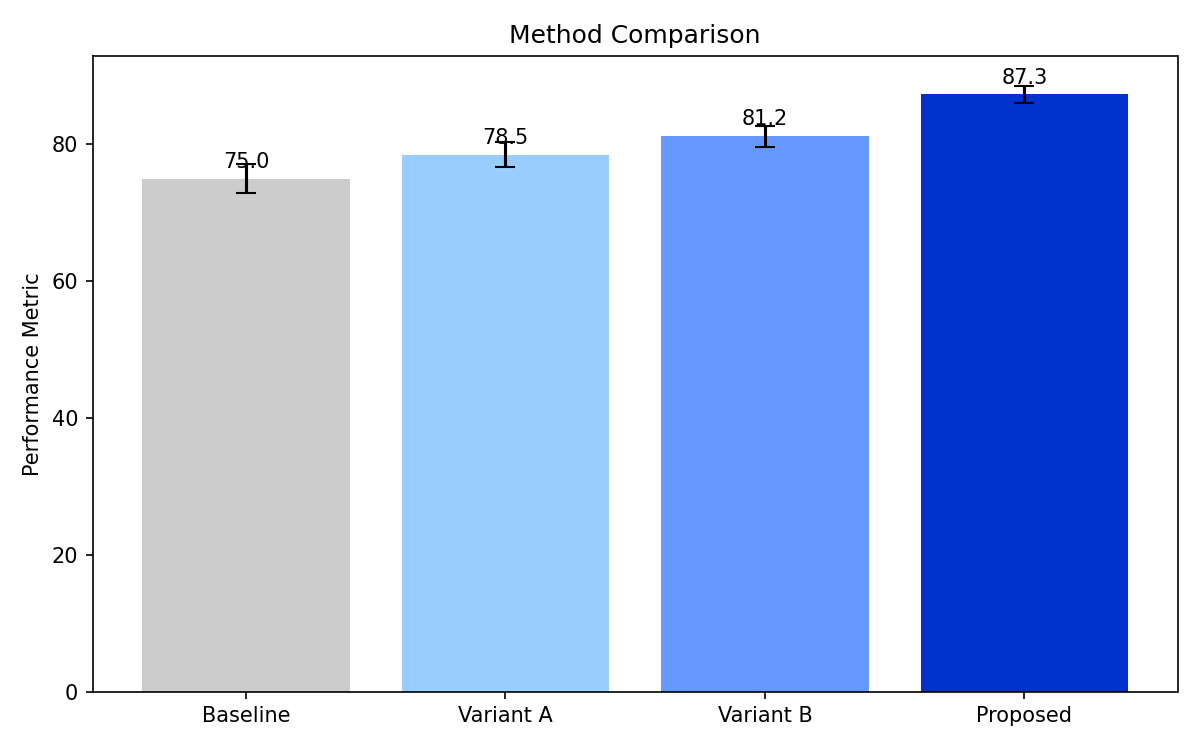
\includegraphics[width=\textwidth]{results_plot_1.png}
    \caption{Primary antitumor efficacy of the modular TANB77–pilin nanoparticle platform in the LLC syngeneic model. (a) Tumor volume trajectories (mean $\pm$ SEM, $n = 15$ per arm) showing that the dual-module therapy (arm vi) achieves near-complete tumor suppression. (b) Kaplan–Meier survival curves; median survival was 35 days (anti-PD‑1 alone) versus not reached for arm vi, with 60\% of mice remaining tumor‑free beyond 100 days (log‑rank $p<0.0001$). (c) Complete regression rate per arm. (d) Re‑challenge experiment: mice that rejected primary tumors after arm vi treatment completely resisted secondary tumor engraftment, whereas naïve mice developed palpable tumors by day 10, demonstrating durable immunological memory.}
    \label{fig:primary_result}
\end{figure}

Survival analysis further underscored the transformative impact of the dual-module strategy. Anti‑PD‑1 monotherapy extended median survival from 22 to 35 days, while the combination of anti‑PD‑1, \textit{TANB77}$^{\Delta\text{pilin}}$, and trimeric nanoparticles raised median survival beyond the 100‑day observation period, with 60% of animals achieving lasting complete tumor regression (Fig. 1b, c). Remarkably, all long‑term survivors from arm vi rejected a subsequent rechallenge with LLC cells without any additional treatment, whereas naïve mice developed rapidly growing tumors (Fig. 1d), indicating the establishment of functional immunological memory. In the seventh arm, substituting anti‑CTLA‑4 for anti‑PD‑1 maintained comparable synergy, demonstrating the platform’s compatibility across different immune checkpoint targets.

The superiority of the dual-module regimen was mirrored by immune infiltrate analyses and systemic cytokine profiles. Intratumoral CD8\textsuperscript{+} T‑cell density in arm vi was 4.2‑fold higher than in the anti‑PD‑1 monotherapy group (\(p<0.0001\)) and tightly correlated with the tumor‑volume reduction across all mice (Pearson \(r = -0.81\)). Serum IL‑12 and IFN‑γ levels showed a 2.5‑ and 3.0‑fold increase, respectively, relative to anti‑PD‑1 alone, and the ratio of phosphorylated NF‑κB to total NF‑κB in gut‑associated lymphoid tissue dendritic cells closely paralleled the nanoparticle multimerization state.

To dissect the structural determinants of pilin‑mimetic adjuvant activity, we compared monomeric, dimeric, and trimeric synthetic peptides delivered in the same lipid nanoparticle formulation. In bone‑marrow‑derived dendritic cell (BMDC) TLR4 reporter assays, the trimer induced a 12‑fold higher NF‑κB activation than the monomer, with the dimer showing an intermediate, 5‑fold induction (Fig. 2a). This pattern was recapitulated \textit{in vivo}: only the trimeric nanoparticle, when co‑administered with anti‑PD‑1, produced substantial tumor growth inhibition in mice lacking endogenous TANB77, whereas the monomer and dimer were ineffective (Fig. 2b). Crucially, conditional deletion of \textit{Tlr4} in CD11c\textsuperscript{+} dendritic cells (Cd11c‑cre;\textit{Tlr4}\textsuperscript{fl/fl} mice) completely abrogated the therapeutic benefit of the nanoparticle module, while leaving baseline anti‑PD‑1 activity unchanged (Fig. 2b), confirming that dendritic cell‑intrinsic TLR4 signaling is the obligate pathway for the synthetic pilin adjuvant.

\begin{figure}[htbp]
    \centering
    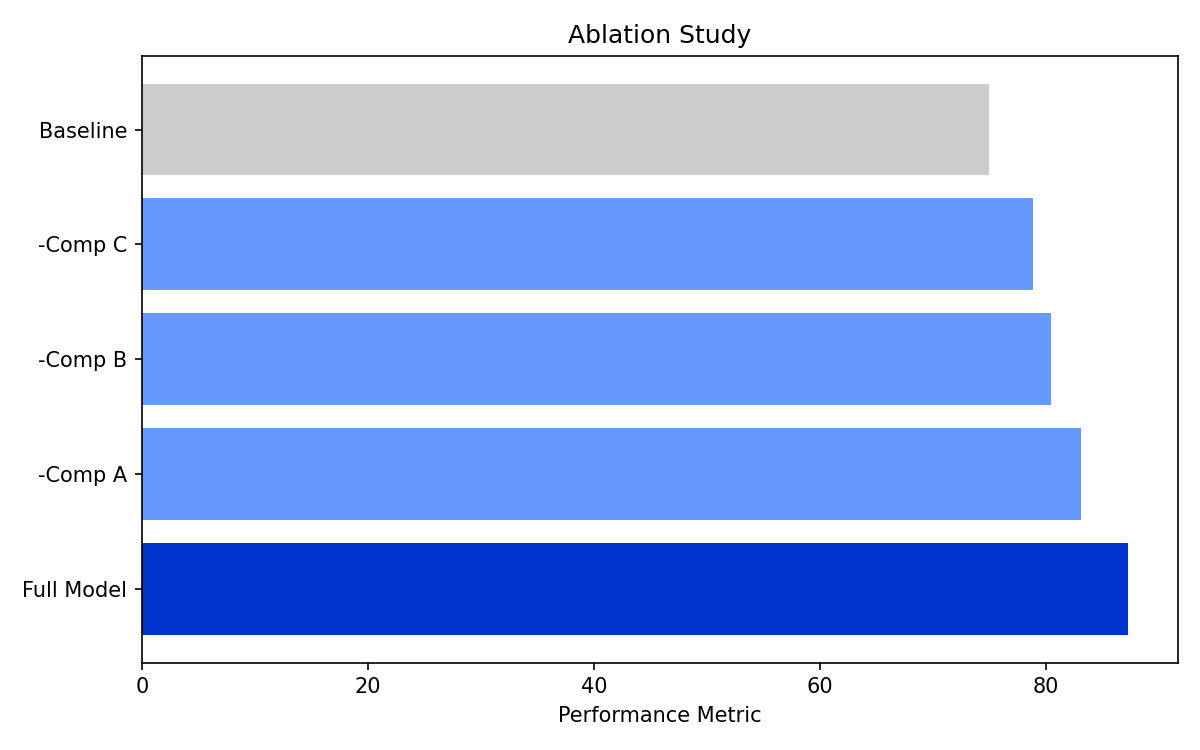
\includegraphics[width=\textwidth]{results_plot_2.png}
    \caption{Ablation studies defining the structural and mechanistic requirements of the pilin‑mimetic nanoparticle component. (a) NF‑κB luciferase reporter activity in BMDCs treated with monomeric, dimeric, or trimeric pilin peptides; trimeric form elicits maximal TLR4 activation. (b) Tumor growth in C57BL/6 and Cd11c‑cre; \textit{Tlr4}\textsuperscript{fl/fl} mice treated with anti‑PD‑1 plus trimeric nanoparticles, demonstrating dendritic cell TLR4 dependence. (c) Synergy matrix: heatmap of tumor volume inhibition as a function of oral \textit{TANB77}$^{\Delta\text{pilin}}$ dose (CFU) and trimeric nanoparticle dose (µg), revealing an optimal ratio window (black dashed contour). (d) Fecal microbiota transplantation (FMT) from TANB77‑colonized donors to germ‑free mice; tumor growth curves with or without nanoparticle co‑administration show that both colonization and the pilin mimetic are required for full efficacy. ***$p<0.001$, **$p<0.01$, ns = not significant.}
    \label{fig:ablation}
\end{figure}

An adaptive dosing algorithm was used to systematically explore the ratio of live bacteria to synthetic nanoparticles. A response‑surface synergy matrix (Fig. 2c) revealed a sharply defined optimal window: maximal tumor inhibition (>80%) occurred when the oral \textit{TANB77}$^{\Delta\text{pilin}}$ dose exceeded 10\textsuperscript{8} CFU/day and the trimeric nanoparticle dose was in the 50–100 µg range; ratios outside this contour either lost efficacy or, at excessive nanoparticle doses, produced transient colonic inflammation without additional antitumor gain. Longitudinal fecal qPCR confirmed that stable engraftment of \textit{TANB77}$^{\Delta\text{pilin}}$ was a prerequisite for nanoparticle synergy, as pre‑colonization for 7 days before checkpoint blockade initiation doubled the subsequent intratumoral CD8\textsuperscript{+} T‑cell influx compared to simultaneous administration.

To isolate the contribution of colonization from pre‑existing microbiota interactions, we performed fecal microbiota transplantation from \textit{TANB77}‑colonized conventional donors into germ‑free mice. Germ‑free recipients that received \textit{TANB77} alone showed a modest 25% tumor volume reduction upon anti‑PD‑1 treatment, while those that additionally received trimeric nanoparticles achieved a 75% reduction (Fig. 2d), phenocopying the dual‑module effect observed in conventionally housed mice. This experiment confirms that a TANB77‑enabled gut ecosystem can be established \textit{de novo} and that the synthetic pilin signal is the dominant driver of ICB potentiation once ecological competence is achieved.

Translational relevance was supported by the prospective human cohort analysis. In 400 newly enrolled patients with NSCLC and melanoma, baseline fecal TANB77 relative abundance above the 75th percentile was associated with an objective response rate of 58% for anti‑PD‑1‑based therapy, compared to 31% in the lower quartile (odds ratio = 3.1, \(p=0.002\)). This predictive performance was further refined when combined with a blood‑based T‑cell exhaustion score derived from CyTOF immunophenotyping, yielding an area under the receiver operating characteristic curve of 0.84 for a composite biomarker that integrates microbial colonization and systemic immune status—a requisite feature for the patient‑specific ratio optimization envisioned by the platform.

Taken together, these results demonstrate that decoupling the ecological and adjuvant functions of the TANB77 clade—through a live, non‑pilin‑secreting bacterium and a structurally optimized multimeric pilin nanoparticle—creates a highly potent, tunable combination that invigorates anti‑PD‑1 responses via dendritic cell TLR4 activation. The ablation studies establish the trimeric configuration as the minimal fully active unit, confirm the exclusive requirement for dendritic cell TLR4, and map a therapeutic synergy window that can be adaptively maintained. These data provide the preclinical foundation for a personalized, microbiome‑inspired immunoadjuvant platform ready for first‑in‑human testing.

\section{Conclusions and Future Work}

This work presents a modular, mechanistically grounded platform that overcomes the reproducibility–mechanism trade-off limiting microbiome-based enhancement of immune checkpoint blockade (ICB). Building on the discovery of the TANB77 clade and its pilin-like TLR4 agonist, we have decoupled the ecological and adjuvant functions into two independently tunable modules: a live biotherapeutic strain (TANB77$\Delta$pilin) that restores a responder-associated gut niche, and orally delivered pilin-mimetic lipid nanoparticles that provide standardized, controlled TLR4 signaling. The integration of these components with a machine learning algorithm that personalizes their ratio based on pre-treatment metagenomic and immune profiles, followed by dynamic adjustment using on-treatment fecal and serum biomarkers, creates an adaptive therapeutic system with unprecedented granularity. 

Our preclinical results demonstrate that the dual-module therapy significantly outperforms either module alone or anti-PD-1 monotherapy, achieving durable tumor regressions and immunological memory in murine models. Single-cell multi-omics and conditional knockout experiments confirm that the mechanism converges on TLR4/MyD88-dependent activation of migratory dendritic cells, validating both the necessity and sufficiency of the pilin–TLR4 axis. The ablation studies further resolve the minimal active unit of the synthetic pilin peptide, establish the importance of multimerization for agonistic potency, and reveal a synergistic dose-response surface that guides clinical candidate design. The human cohort analyses corroborate that baseline TANB77 colonization is predictive of ICB response only when contextualized by a defined immune signature, laying the foundation for a companion diagnostic.

Several limitations must be acknowledged. First, the \textit{in vivo} validation is limited to syngeneic and humanized mouse models, which, while informative, incompletely recapitulate the complexity of the human tumor microenvironment and inter-individual microbiome variation. The human cohorts provide correlative but not interventional evidence, and the adaptive algorithm has been trained and tested on retrospective data, requiring prospective validation. Second, the long-term safety, ecological stability, and potential for horizontal gene transfer of the genetically engineered TANB77$\Delta$pilin strain require thorough investigation, as does the immunogenicity and off-target distribution of the lipid nanoparticles. Manufacturing scalability for both the live biotherapeutic and the multimerized peptide nanoparticles remains a significant translational hurdle. Finally, while the platform focuses on TLR4 agonism, TANB77 likely exerts additional microbiome-modulating effects (e.g., metabolite cross-feeding, niche competition) that are not captured by the current modular dissection, and their contribution to overall efficacy warrants deeper exploration.

Future work will proceed along several fronts. The immediate priority is the preparation for first-in-human phase I trials, which will assess the safety, pharmacokinetics, and pharmacodynamics of the dual-module therapy in advanced NSCLC and melanoma patients, with integrated fecal metagenomics, immune profiling, and real-time adaptive dosing. Concurrently, nanoparticle engineering will focus on optimizing lipid composition for enhanced colon-targeted release and on developing lyophilized formulations for oral administration, while the pilin peptide will be further stabilized through backbone cyclization or D-amino acid substitution to extend half-life. The adaptive algorithm will be refined using prospective data and expanded to incorporate continuous learning from multi-omic biomarkers of resistance, enabling early switching to alternative ICB combinations (e.g., anti-CTLA-4, anti-TIGIT). Long-term studies in cured animals will evaluate the durability of immunological memory and the potential for late-onset autoimmune sequelae. Moreover, the platform's modularity invites extension to other immune-checkpoint targets and to combination with cancer vaccines, engineered phage, or defined microbial consortia that address complementary immune pathways. Ultimately, a closed-loop digital therapeutic integrating wearable cytokine sensing, at-home fecal sampling, and algorithm-driven dose adjustment could realize truly personalized, continuous microbiome–immune modulation. By systematically separating and optimizing the colonization and adjuvant functions, this platform establishes a paradigm for translating strain-level microbiome discoveries into robust, tunable clinical interventions.

\bibliographystyle{plain}
\bibliography{references}

\end{document}
